\documentclass[a4paper,12pt]{article}
\usepackage[ukrainian,english]{babel}
\usepackage{ucs}
\usepackage[utf8]{inputenc}
\usepackage[T2A]{fontenc}
\usepackage{amsmath}
\usepackage{amsfonts}
\usepackage{graphicx}
\usepackage{changepage}
\usepackage{multirow}
\usepackage{subcaption}
\usepackage{array, makecell}
\usepackage[document]{ragged2e}
\usepackage{parskip}
\usepackage[paper=portrait,pagesize]{typearea}
\usepackage{multicol}
\newcommand\tab[1][1cm]{\hspace*{#1}}
\addto\captionsenglish{\renewcommand{\figurename}{Рис.}}
\addto\captionsenglish{\renewcommand{\tablename}{Таблиця}}
\captionsetup[table]{justification=raggedleft,singlelinecheck=off}
\usepackage{titlesec}
\usepackage[left=20mm, top=20mm, right=20mm, bottom=20mm, nohead, nofoot]{geometry}
\titleformat{\section}[block]{\Large\bfseries\filcenter}{}{1em}{}
\titleformat{\subsection}[hang]{\bfseries}{}{1em}{}
\titleformat{\subsubsection}[hang]{\bfseries}{}{2em}{}
\begin{document}
\begin{justify}
\thispagestyle{empty}\setlength{\parindent}{0pt}
	\begin{center}
		\textbf{НАЦІОНАЛЬНИЙ ТЕХНІЧНИЙ УНІВЕРСИТЕТ УКРАЇНИ}\\ 
		\textbf{«КИЇВСЬКИЙ ПОЛІТЕХНІЧНИЙ ІНСТИТУТ»}\\ 
		\textbf{ФІЗИКО-ТЕХНІЧНИЙ ІНСТИТУТ}
	\end{center}
	$\\\\\\\\\\\\\\\\\\\\\\\\\\$
	\begin{center}
		Лабораторна робота з фізики №1\bigbreak
ВНУТРІШНІЙ ОПІР ДЖЕРЕЛ ЕЛЕКТРИЧНОЇ ЕНЕРГІЇ ТА УЗГОДЖЕННЯ ПОТУЖНОСТЕЙ

	\end{center}
	$\\\\\\\\\\\\\\\\\\\\\\\\\\$
	\begin{flushright}
	Виконалa:\\
		студент групи ФІ-12\\
		Бекешева Анастасія 
	\end{flushright}
	$\\\\\\\\\\$
	\begin{center}
		\textbf{Київ-2022}
	\end{center}
	\newpage
	\section{Розділ 1. Теоретична довідка.}
	\textbf{Ключові поняття:}  джерело струму або напруги, електрорушійна сила, ЕРС, вихідна напруга, напруга на клемах джерела, холостий хід, робота без навантаження, коротке замикання, закон Ома, закони Кірхгофа, узгодження потужностей.\bigbreak
	\textbf{Мета роботи:} Дослідити декілька джерел електричної енергії на предмет: 
	\begin{itemize}
		\item Внутрішнього опору;
		\item Узгодження потужностей джерела та споживача;
		\item Визначити до якої групи відноситься те чи інше джерело за величиною внутрішнього опору (джерело напруги або джерело струму);
		\item Визначити за якого режиму джерело буде віддавати максимальну корисну потужність;
		\item За якого режиму джерело матиме максимальний ККД.
	\end{itemize}
	\subsection{Теоретичне підгрунтя:}
	Розглянемо електричне коло \figurename{\ref{fig:1}} , яке складається з джерела електричної енергії зі своїм внутрішнім незмінним опором $R_i$, з зовнішнього опору навантаження(реостат) $R_e$, який можна змінювати, амперметра $А$ та вольтметра $V$.
	\begin{figure*}[!h]
		\centering
		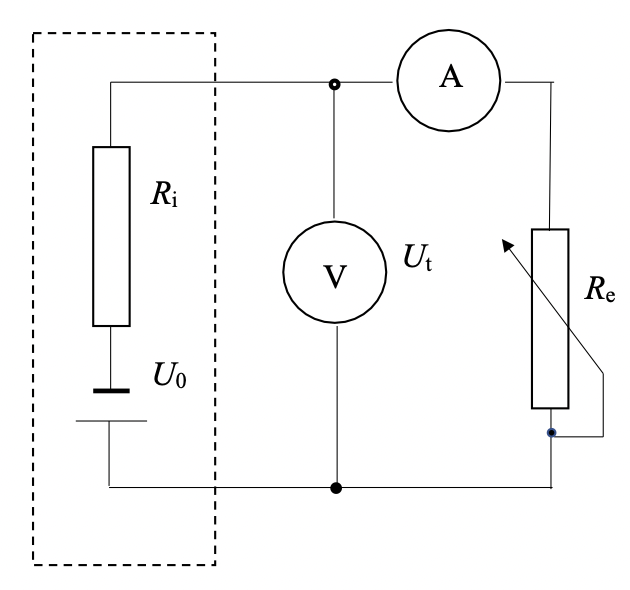
\includegraphics[height=50mm]{media/graph1.png}
		\caption{Схема електричного кола}
		\label{fig:1}
	\end{figure*}\\
	Струм у колі визначається за сумою опору навантаження $R_e$ та внутрішнього опору $R_i$. Так як опір $R_i$ є незмінним, то зміна струму в колі залежить від величини опору навантаження $R_e$ і визначається за рівнянням закону Ома: $$I=\dfrac{U_0}{R_i+R_e}$$
	Приймає найменше значення $І = 0$ при $R_e = \infty$, та найбільше при $R_e=0$
	\begin{itemize}
		\item Режим кола, коли опір навантаження $R_e=\infty$ визначається як \textbf{режим холостого ходу}. Тобто на клемах джерела присутня напруга холостого ходу $U_0$.
		\item Режим кола, коли опір навантаження $R_e= 0$ визначається як \textbf{режим короткого замикання}, струм в колі максимальний.
	\end{itemize}\newpage
	Прослідкуємо як змінюються спад напруги на опорах в залежності від струму в колі.\\ 
	Спад напруги на внутрішньому опорі дорівнює:
	$$U_{R_i}=I\cdot R_i$$
	Величина цього спаду напруги пропорційна величині струму і змінюється від 0 до найбільшого значення $U_0$ при струму максимальному.\\
	Спад напруги на зовнішньому опорі дорівнює:
	$$I\cdot R_e=U_0-I\cdot R_i$$
	Цей спад напруги також знаходиться в лінійній залежності від струму. Так як опір навантаження під’єднаний до вихідних клем джерела, то спад напруги на опорі навантаження можна вважати як вихідну напругу джерела яка визначається за рівнянням:
	$$U_{R_e}=U_0-U_{R_i}$$
	Нормовані графіки, які показують залежність $U_{R_i}$ та $U_{R_e}$ від струму $І$ наведенні на рис. 2
	\begin{figure*}[!h]
		\centering
		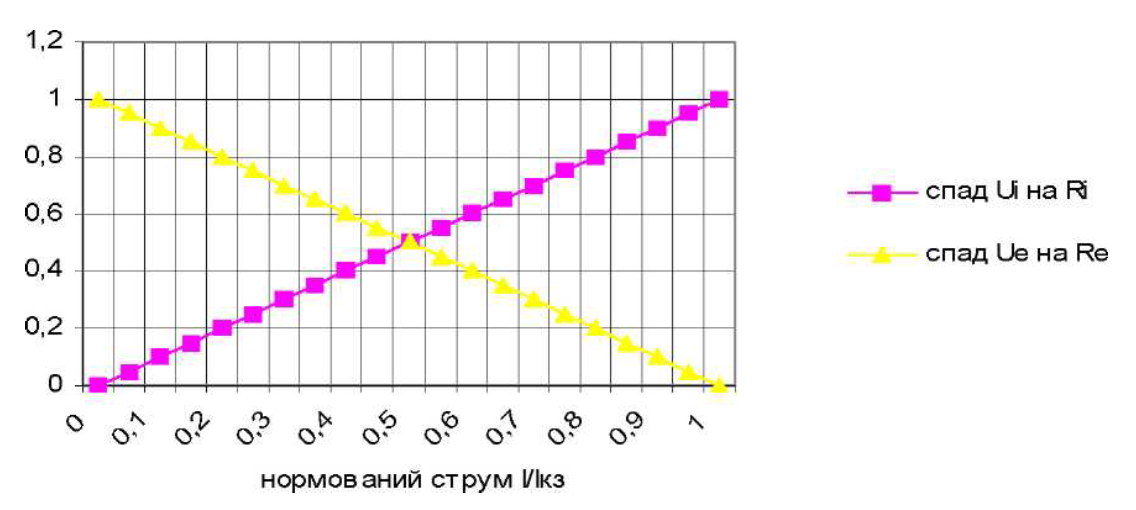
\includegraphics[height=50mm]{media/graph2.png}
		\caption{}
		\label{fig:2}
	\end{figure*}\\
	За умов коли $R_e=R_i$, а їхня сума дорівнює $2R$, має місце співвідношення:
	$$I=\dfrac{U_0}{2R}=\dfrac{I_{\textrm{кз}}}{2}$$
	І спад напруг на опорах рівні між собою, тобто:
	$$\dfrac{I_{\textrm{кз}}}{2}\cdot R_i=\dfrac{I_{\textrm{кз}}}{2}\cdot R_e=\dfrac{U_0}{2}$$
	Такий режим називається узгодження внутрішнього опору джерела та опору споживача, або узгодженням потужностей джерела та споживача.
	електрична потужність визначається за співвідношеням:
	$$P=R\cdot I^2=\dfrac{U^2}{2}$$ 
	Визначимо співвідношення між потужностями, які виділяються на елементах електричного кола.\\
	Повна потужність електричного кола визначається за співвідношенням:
	$$P_0=U_0\cdot I_{\textrm{кз}}$$\newpage
	Повна потужність джерела складається з потужності, яка виділяється на внутрішньому опорі джерела визначається за співвідношенням:
	$$P_i=I^2\cdot R_i$$
	Потужність, яка виділяється на опорі навантаження
	$$P_e=I^2\cdot R_e$$
	Визначається як різниця між повною потужністю та потужністю, яка виділяється на внутрішньому опорі
	$$P_e=P_0-P_i=U_0\cdot I_{\textrm{кз}}-I^2R_i$$
	Потужність джерела струму змінюється пропорційно струму від найменшого значення до найбільшого.\\
	Потужність дорівнює нулю, коли струм дорівнює нулю. Для визначення найбільшого значення потужності візьмемо першу похідну від минулої формули та прирівнемо її до 0. Звідти отримаємо співвідношення:
	$$U_0=2I\cdot R_i$$
	Але при будь-якому значенні опору $R_e$(при будь-якому режимі)
	$$U_0=I\cdot(R_i+R_e)$$
	Порівнюючи два останні вирази видно, що потужність $P_e$ досягає найбільшого значення при $R_i=R_e$, струм в колі буде відповідати:
	$$I=\dfrac{U_0}{2R_i}=\dfrac{I_{\textrm{кз}}}{2}$$
	Тобто максимальна потужність $P_e$, яка виділяється на зовнішньомуопорі навантаження буде дорівнювати потужності $P_i$, яка виділяється на внутрішньому опорі і буде дорівнювати $\frac14 P_0$ – режим узгодження потужностей джерела та споживача.
	$$P_e=I^2\cdot R_e=\dfrac{U_0^2}{4R_i^2}$$
	Графіки, які виявляють залежність потужностей від відношення опорів наведенні на \ref{fig:3} та \ref{fig:4}
	\begin{figure*}[!h]
		\centering
		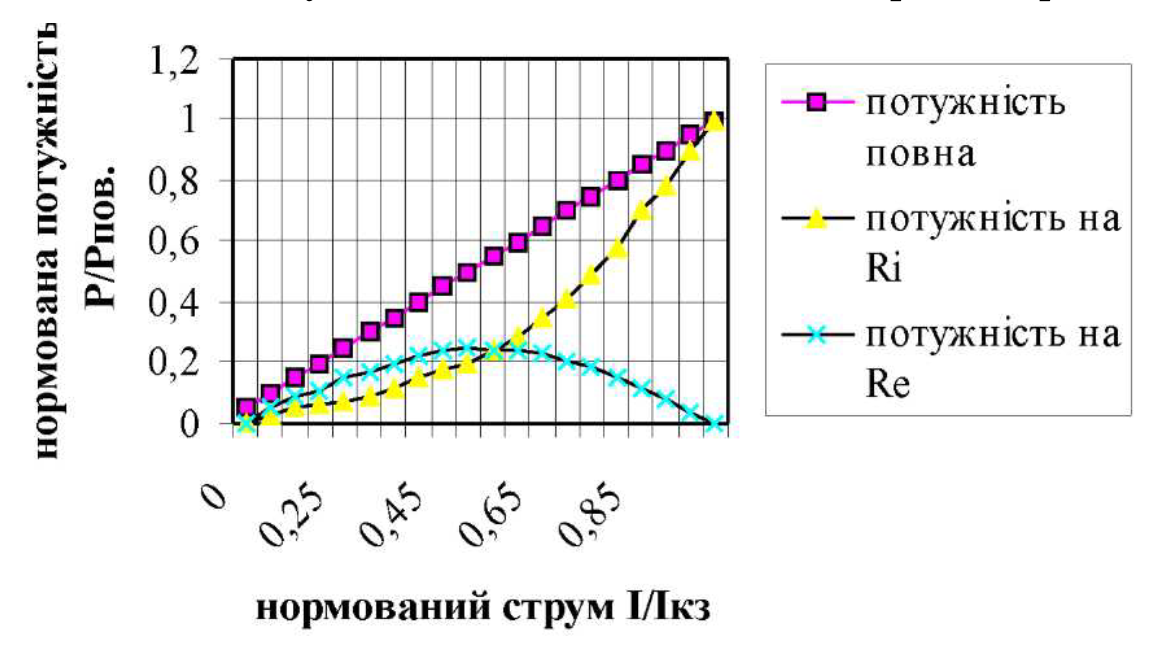
\includegraphics[height=50mm]{media/graph3.png}
		\caption{Нормованні графіки залежності потужності, які виділяються на опорах $R_i$ та $R_e$ }
		\label{fig:3}
	\end{figure*}\newpage
	\begin{figure*}[!h]
		\centering
		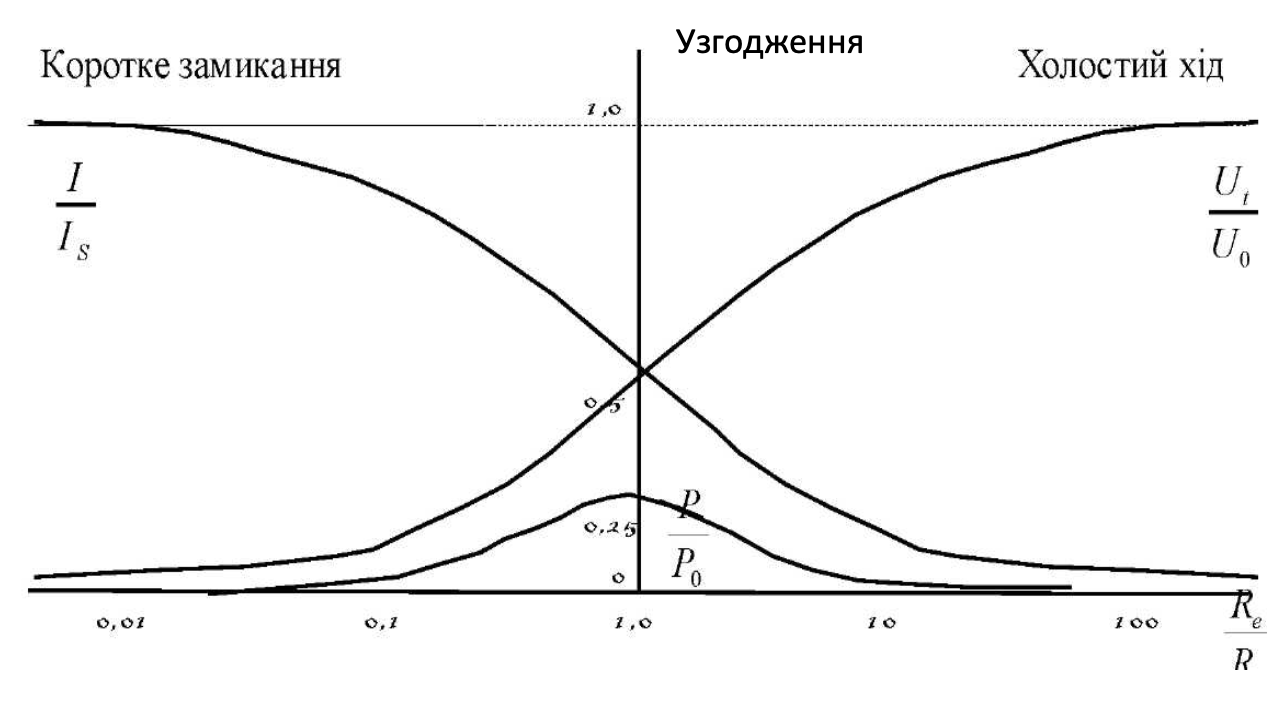
\includegraphics[height=50mm]{media/graph4.png}
		\caption{Нормований графік залежності потужності джерела струму від навантаження}
		\label{fig:4}
	\end{figure*}
	Визначимо за якого режиму джерело видає максимальну корисну потужність. 
	Корисна потужність – це потужність, яка виділяється на опорі навантаження, тобто потужність $P_e$. Потужність, яка виділяється на внутрішньому опорі, це потужність втрат $Pi.$ \\
	Режим, коли джерело розвиває найбільшу корисну потужність має місце при:
	$$R_i=R_e$$
 	В цьому випадку струм у колі дорівнює струм короткого замикання поділений на 2, а корисна потужність і потужність втрат дорівнює
 	$$P_i=P_e=\dfrac{U_0\cdot I_{\textrm{кз}}}{4}$$
 	Максимальна потужність, яку може розвинути джерело:
 	$$P_0=-U_0\cdot I_{\textrm{кз}}$$
	К.К.Д – коефіцієнт корисної дії джерела визначається як відношення корисної потужності, виділеної на навантаженні до повної потужності. Як видно з \ref{fig:3} та \ref{fig:4} корисна потужність дорівнює 0.25 від повної потужності джерела. Потужність, яку розвине джерело в режимі узгодження дорівнює сумі потужностей на внутрішньому та зовнішньому опорі і дорівнює 0.5 повної потужності. Тобто ККД за режиму узгодження коли $P_i = P_e$ джерела дорівнює: 
	$$\eta=\dfrac{P_e+P_i}{P_0}=\dfrac12$$
	\subsection{Експериментальне обладнання:}
	Експериментальне обладнання складається з трьох джерел електричної енергії:
	\begin{itemize}
		\item Батарейка з трьох марганцево-цинкових елементів для кишенькових ліхтариків;
		\item Свинцевого кислого акумулятора;
		\item Електронного блока живлення;
		\item Реостата з максимальним опором 10 Ом;
		\item Реостата з максимальним опором 45 Ом;
		\item Реостата з максимальним опором 100 Ом;
		\item Астатичний амперметра
		\item Цифрового вольтметра
		\item В якості амперметра використовується магнітоелектричний прилад. В якості вольтметра використовується вольтметра з великим вхідним опором.

	\end{itemize}
	\subsection{Хід експеременту.}
	\subsubsection{Дослід №1}
	\begin{enumerate}
		\item Зберіть вимірювальну схему згідно \ref{fig:1} (в якості джерела використайте марганцево-цинкову батарейку для кишенькового ліхтарика)
		\item В якості навантаження використати реостат з максимальним опором 45 або 100 Ом.
		\item Виміряти напругу холостого ходу – $U_0$ (на клемах джерела без навантаження)
		\item За допомогою вольтметра виміряти залежності напруги $U_{R_e}$ на опорі навантаження від струму $І$, тобто від величини опору навантаження (струм змінювати реостат з кроком 0.1 А до максимального значення 2А, тобто зробити 15-20 вимірів).
		\item Встановіть опір навантаження таким, щоб спад напруги на опорі навантаження $U_{R_e}$ становить $\frac12 U_0$. В цьому випадку опір навантаження буде дорівнювати внутрішньому опору джерела $R_e=R_i$(режим узгодження опорів або потужностей). Не змінюючи положення реостата за допомогою омметра виміряйте опір навантаження.
		\item Отримані дані занесіть до таблиці.
	\end{enumerate}
	\subsubsection{Дослід №2}
	\begin{enumerate}
		\item Зберіть вимірювальну схему згідно \ref{fig:1} (в якості джерела використайте свинцевий акумулятор) 
		\item В якості навантаження використати реостат з максимальним опором 45 або 100 Ом.
		\item Виміряти напругу холостого ходу – $U_0$ (на клемах джерела без навантаження).
		\item Виміряти залежності напруги $U_{R_e}$ від струму $І$, тобто від величини навантаження (струм змінювати реостатом з кроком 0.05 – 0.1А до максимального значення 2А, зробити 10 –15 вимірів).
		\item Отримані дані занесіть до таблиці.
	\end{enumerate}
	\subsubsection{Дослід №3}
	\begin{enumerate}
		\item Зберіть вимірювальну схему згідно \ref{fig:1} (в якості джерела використайте блок живлення, який живиться від силової мережі).
		\item В якості навантаження використати реостат з максимальним опором 45 або 100 Ом.
		\item Виміряти напругу холостого ходу – $U_0$ (на клемах джерела без навантаження).
		\item За допомогою вольтметра для кожного значення струму виміряйте залежність спаду напруги на опорі навантаження $U_{R_e}$ від струму $І$, тобто від величини опору навантаження (струм змінювати реостат з кроком 0.1А до максимального значення 2А, тобто зробити 15-20 вимірів)
		\item Отримані дані занесіть до таблиці.
	\end{enumerate}
	\subsection{Завдання.}
	\begin{enumerate}
		\item Побудуйте графік залежності $U(I)$ для всіх досліджуваних джерел. Зробіть аппроксимацию для кожного побудованого графіка.
		\item За апроксимацією графіків визначте внутрішній опір кожного джерела за різних режимів навантаження.
		\item Побудуйте нормовані графіки залежності потужності від струму аналогічно \ref{fig:3} та \ref{fig:4}.
		\item Визначте похибки, поясніть за яких факторів виникли ці похибки..
		\item На підставі проведених дослідів та розрахунків дайте остаточну характеристику кожного з джерел та зробіть висновки.
	\end{enumerate}
	\newpage
	\section{Розділ 2. Експерементальні дані.}

	\begin{figure*}[!h]
		\centering
		\begin{subfigure}{0.6\linewidth}
			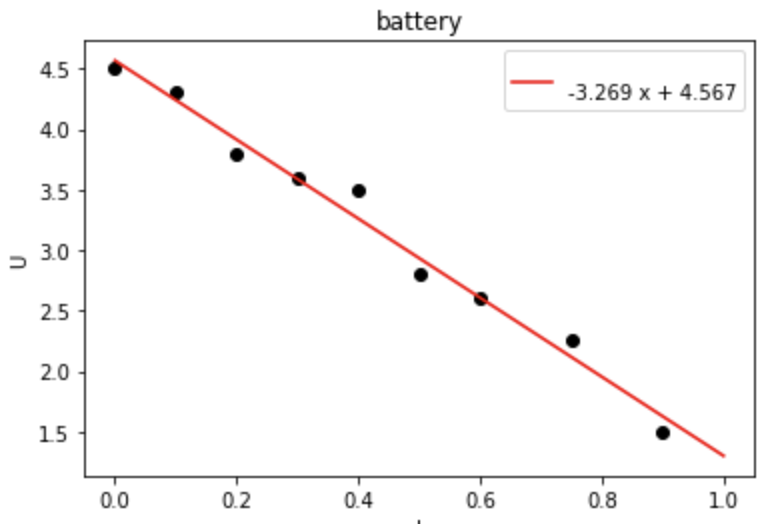
\includegraphics[height=65mm]{media/graph6aa.png}
    		\caption{Батарейка}
			\label{fig:6a}
    	\end{subfigure}\hfill
    	    	\begin{subfigure}{0.6\linewidth}
			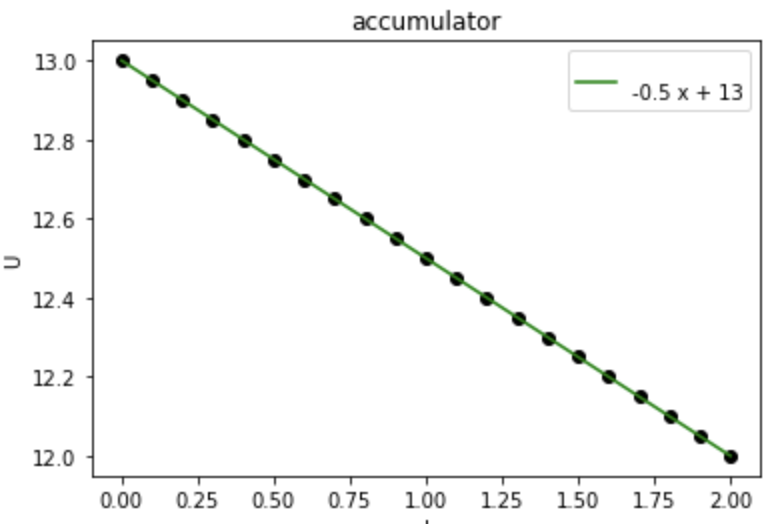
\includegraphics[height=65mm]{media/graph6bb.png}
    		\caption{Акумулятор}
			\label{fig:6b}
    	\end{subfigure}\hfill
    	\begin{subfigure}{0.6\linewidth}
			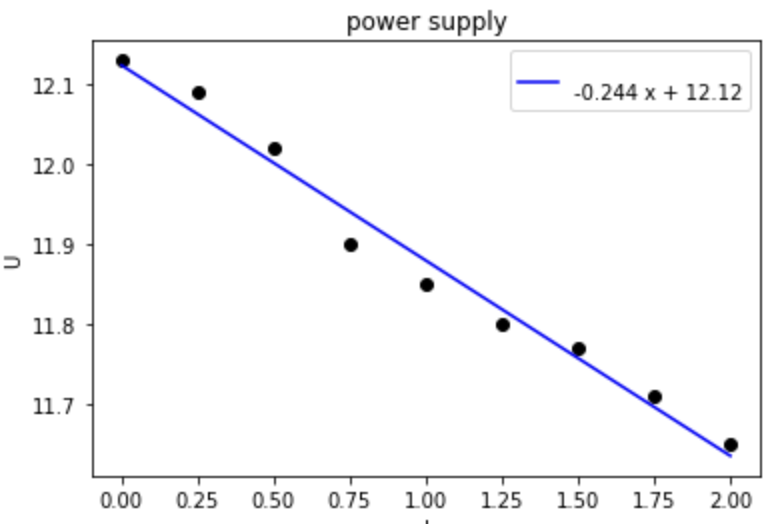
\includegraphics[height=65mm]{media/graph6cc.png}
    		\caption{Блок живлення}
			\label{fig:6c}
    	\end{subfigure}\hfill
		\caption{Апроксимовані графіки залежності $U$ від $I$}
		\label{fig:6}
	\end{figure*}$\\$
	\subsection{Внутрішній опір.}
	\begin{itemize}
		\item З графіку \ref{fig:6a} лінійна апроксимація залежності $U$ від $I$ батарейки: $$y=-3.269 x + 4.567$$ А отже $R_i$ апроксимоване дорівнює $3.329$
		\item З графіку \ref{fig:6b} лінійна апроксимація залежності $U$ від $I$ акумулятору: $$y=-0.5 x + 13$$  А отже $R_i$ апроксимоване дорівнює $0.5$
		\item З графіку \ref{fig:6b} лінійна апроксимація залежності $U$ від $I$ блоку живлення: $$y=-0.244 x + 12.12$$ А отже $R_i$ апроксимоване дорівнює $0.2414$
	\end{itemize}\subsection{Похибки.}
	Похибки та усереднені значення будуть обчислюватись за такими формулами:
	\begin{equation}\label{eq:p1}
		\langle R_i\rangle=\dfrac1n\sum_{k=1}^{n}R_{i_k}
	\end{equation}
	\begin{equation}\label{eq:p2}
		\Delta R_i=\sqrt{(\Delta R_r)^2+(\Delta R_s)^2},\>R_r=\sqrt{\dfrac{\displaystyle\sum_{k=1}^{n}(R_{i_k}-\bar{R_i})^2}{n(n-1)}},\>\bar{R_i}=\dfrac{R_{i_1}+R_{i_2}+\dots+R_{i_n}}{n}
	\end{equation}	
	\begin{equation}\label{eq:p3}
		\varepsilon_{R_i}=\dfrac{\Delta R_i}{\bar{R_i}},\>\bar{R_i}=\dfrac{R_{i_1}+R_{i_2}+\dots+R_{i_n}}{n}
	\end{equation}
	\begin{itemize}
		\item За формулою \ref{eq:p1}: $$\textrm{Батарейка: }\langle R_i\rangle=2.99 \textrm{ Ом}$$ $$\textrm{Акумулятор: }\langle R_i\rangle=0.5\textrm{ Ом}$$ $$\textrm{Блока живлення: }\langle R_i\rangle=0.24\textrm{ Ом}$$
		\item За формулою \ref{eq:p2}: $$\textrm{Батарейка: }\Delta R_i=0.18\textrm{ Ом}$$ $$\textrm{Акумулятор: }\Delta R_i=0.0\textrm{ Ом}$$ $$\textrm{Блока живлення: }\Delta R_i=0.15\textrm{ Ом}$$
		\item За формулою \ref{eq:p3}: $$\textrm{Батарейка: }\varepsilon_{R_i}=0.06\textrm{ Ом}$$ $$\textrm{Акумулятор: }\varepsilon_{R_i}=0.0\textrm{ Ом}$$ $$\textrm{Блока живлення: }\varepsilon_{R_i}=0.06\textrm{ Ом}$$
	\end{itemize}
	Похибки виникли через неточність вимірюваня(людський фактор). 
\newpage
	\subsection{Нормовані графіки залежності потужності і струму.}
	 \begin{figure*}[!h]
		\centering
		\begin{subfigure}{0.6\linewidth}
			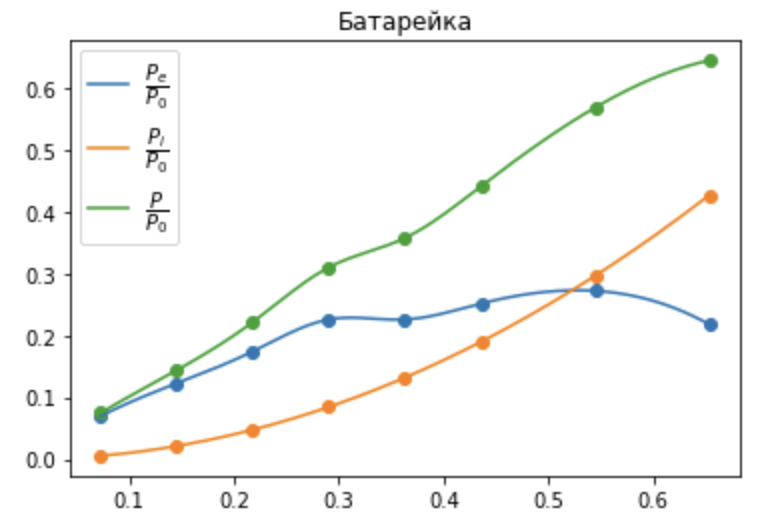
\includegraphics[height=65mm]{media/graph7aaaa.png}
    		\caption{Батарейка}
			\label{fig:8a}
    	\end{subfigure}\hfill

		\caption{Нормовані графіки залежності потужності джерела від навантаження}
		\label{fig:8}
	\end{figure*}
		
	\subsection{Висновки}	
	Мета лаборотарної роботи полягала у дослідженні опору, сили струму, напруги, потужності, ККД в електричному полі. Протягом роботи також були досліджені питання властивостей електричного поля та поведінки струму. \\Після обробки даних та необхідних підрахунків було визначено залежності напруг на клемах джерел струму від сили струму. Всього було побудовано три залежності: для батарейки, акумулятора та блоку живлення. 
	\begin{itemize}
		\item Батарейка: $R_i=3.269$ Ом, $U_0=4.5$ В.
		\item Акумулятор: $R_i=0.5$ Ом, $U_0=13$ В.
		\item Блок живлення: $R_i=0.244$ Ом, $U_0=12.13$ В.
	\end{itemize} 
	На \ref{fig:5} та \ref{fig:6} рисунах спостерігається лінійна залежність напруги від сили струму. З них можна зробити висновок, що  внутрішні опори $R_i$ джерел струму і напруги є сталими. \\
	На \ref{fig:8} рисунку було показано нормована залежність зміни потужностей від струму для таких джерел: батарейка, акумулятор та блок живлення. Легко бачити, що при збільшенні струму, збільшуєтся потужність джерела. Після обрахуну внутрішнього $R_i$ та зовнішнього $R_e$ опорів можна зазначити, що батарейка є джерелом напруги, акумулятор - джерело напруги (може бути й джерелом струму, але далеко не найкращим), блок живлення може бути, як і джерелом напруги, так і джерелом напруги(але конкретно блок живлення у цьому експеременті не є гарним джерелом струму). 
	\subsection{Умови}
	Чи буде джерело джерелом струму а бо напруги можна визначити дослідивши його внутрішній на зовнішній опір. Якщо зовнішній $R_e$ опір набагато більший за внутрішній $R_i$, то джерело є джерелом напргу, якщо навпаки - джерелом струму.
	
\end{justify}


	\newpage
	\KOMAoptions{paper=landscape,pagesize}
	\recalctypearea
	\section{Таблиці}
	% Please add the following required packages to your document preamble:
% \usepackage{multirow}

% Please add the following required packages to your document preamble:
% \usepackage{multirow}
\begin{table}[htp]\centering
	\label{table:battery}
	\begin{flushright}
		\caption{Батарейка}
	\end{flushright}	
\begin{adjustwidth}{-2cm}{}
\begin{tabular}{|c|c|c|c|c|c|c|c|c|c|c|c|c|c|c|c|c|c|c|c|c|}

\hline
  & \makecell{$U_0$,\\  В} & \makecell{$I$, \\  А} & \makecell{$U$,\\  В} & \makecell{$R_i$ (approx)\\  Ом} & \makecell{$R_i$,\\  Ом} & \makecell{$R_e$,\\  Ом} & \makecell{$U_i$,\\  В} & \makecell{$U_e$,\\  В} & \makecell{$P_e$, \\  Вт} & \makecell{$P_i$, \\  Вт} & \makecell{$I_{kz}$,\\  А} &\makecell{ $P_0$, \\  Вт} & $\dfrac{P_e}{P_0}$ & $\dfrac{P_i}{P_0}$ & \makecell{$P$, \\  Вт} & $\dfrac{P}{P_0}$ & \makecell{ККД, \\  \textrm{ Ом}} & \makecell{$\langle R_i\rangle$, \\  Ом} & \makecell{$\Delta_{R_i}$, \\  \textrm{ Ом}} & \makecell{$\varepsilon_{R_i}$, \\  \textrm{ Ом}} \\ \hline00     & \multirow{8}{*}{4.5} & 0.1  & 4.3  & \multirow{8}{*}{3.27} & 2.0  & 43.0 & 0.33 & 4.17 & 0.43 & 0.03 & \multirow{8}{*}{1.38} & \multirow{8}{*}{6.2} & 0.07      & 0.01      & 0.46 & 0.07   & 6.94       & \multirow{8}{*}{2.99} & \multirow{8}{*}{0.18} & \multirow{8}{*}{0.06} \\ \cline{1-1} \cline{3-4} \cline{6-11} \cline{14-18}
1     &                      & 0.2  & 3.8  &                       & 3.5  & 19.0 & 0.65 & 3.85 & 0.76 & 0.13 &                       &                      & 0.12      & 0.02      & 0.89 & 0.14   & 12.27      &                       &                        &                      \\ \cline{1-1} \cline{3-4} \cline{6-11} \cline{14-18}
2     &                      & 0.3  & 3.6  &                       & 3.0  & 12.0 & 0.98 & 3.52 & 1.08 & 0.29 &                       &                      & 0.17      & 0.05      & 1.37 & 0.22   & 17.43      &                       &                        &                      \\ \cline{1-1} \cline{3-4} \cline{6-11} \cline{14-18}
3     &                      & 0.4  & 3.5  &                       & 2.5  & 8.75 & 1.31 & 3.19 & 1.4  & 0.52 &                       &                      & 0.23      & 0.08      & 1.92 & 0.31   & 22.6       &                       &                        &                      \\ \cline{1-1} \cline{3-4} \cline{6-11} \cline{14-18}
4     &                      & 0.5  & 2.8  &                       & 3.4  & 5.6  & 1.63 & 2.87 & 1.4  & 0.82 &                       &                      & 0.23      & 0.13      & 2.22 & 0.36   & 22.6       &                       &                        &                      \\ \cline{1-1} \cline{3-4} \cline{6-11} \cline{14-18}
5     &                      & 0.6  & 2.6  &                       & 3.17 & 4.33 & 1.96 & 2.54 & 1.56 & 1.18 &                       &                      & 0.25      & 0.19      & 2.74 & 0.44   & 25.18      &                       &                        &                      \\ \cline{1-1} \cline{3-4} \cline{6-11} \cline{14-18}
6     &                      & 0.75 & 2.25 &                       & 3.0  & 3.0  & 2.45 & 2.05 & 1.69 & 1.84 &                       &                      & 0.27      & 0.3       & 3.53 & 0.57   & 27.24      &                       &                        &                      \\ \cline{1-1} \cline{3-4} \cline{6-11} \cline{14-18}
7     &                      & 0.9  & 1.5  &                       & 3.33 & 1.67 & 2.94 & 1.56 & 1.35 & 2.65 &                       &                      & 0.22      & 0.43      & 4.0  & 0.65   & 21.79      &                       &                        &                      \\ \hline\end{tabular}
	\end{adjustwidth}

\end{table}	

% Please add the following required packages to your document preamble:
% \usepackage{multirow}
\begin{table}[htp]
\label{table:ps}
	\caption{Блок живлення}
\begin{adjustwidth}{-2.6cm}{}
\begin{tabular}{|c|c|c|c|c|c|c|c|c|c|c|c|c|c|c|c|c|c|c|c|c|}
\hline
  & \makecell{$U_0$,\\  В} & \makecell{$I$, \\  А} & \makecell{$U$,\\  В} & \makecell{$R_i$ (approx)\\  Ом} & \makecell{$R_i$,\\  Ом} & \makecell{$R_e$,\\  Ом} & \makecell{$U_i$,\\  В} & \makecell{$U_e$,\\  В} & \makecell{$P_e$, \\  Вт} & \makecell{$P_i$, \\  Вт} & \makecell{$I_{kz}$,\\  А} &\makecell{ $P_0$, \\  Вт} & $\dfrac{P_e}{P_0}$ & $\dfrac{P_i}{P_0}$ & \makecell{$P$, \\  Вт} & $\dfrac{P}{P_0}$ & \makecell{ККД, \\  \textrm{ Ом}} & \makecell{$\langle R_i\rangle$, \\  Ом} & \makecell{$\Delta_{R_i}$, \\  \textrm{ Ом}} & \makecell{$\varepsilon_{R_i}$, \\  \textrm{ Ом}} \\ \hline0     & \multirow{8}{*}{12.13} & 0.25 & 12.09 & \multirow{8}{*}{0.24} & 0.16 & 48.36 & 0.06 & 12.07 & 3.02  & 0.02 & \multirow{8}{*}{49.71} & \multirow{8}{*}{603.02} & 0.01      & 0.0       & 3.04  & 0.01   & 0.5        & \multirow{8}{*}{0.24} & \multirow{8}{*}{0.15} & \multirow{8}{*}{0.06} \\ \cline{1-1} \cline{3-4} \cline{6-11} \cline{14-18}
1     &                        & 0.5  & 12.02 &                       & 0.22 & 24.04 & 0.12 & 12.01 & 6.01  & 0.06 &                        &                         & 0.01      & 0.0       & 6.07  & 0.01   & 1.0        &                       &                       &                       \\ \cline{1-1} \cline{3-4} \cline{6-11} \cline{14-18}
2     &                        & 0.75 & 11.9  &                       & 0.31 & 15.87 & 0.18 & 11.95 & 8.93  & 0.14 &                        &                         & 0.01      & 0.0       & 9.06  & 0.02   & 1.48       &                       &                       &                       \\ \cline{1-1} \cline{3-4} \cline{6-11} \cline{14-18}
3     &                        & 1.0  & 11.85 &                       & 0.28 & 11.85 & 0.24 & 11.89 & 11.85 & 0.24 &                        &                         & 0.02      & 0.0       & 12.09 & 0.02   & 1.97       &                       &                       &                       \\ \cline{1-1} \cline{3-4} \cline{6-11} \cline{14-18}
4     &                        & 1.25 & 11.8  &                       & 0.26 & 9.44  & 0.3  & 11.83 & 14.75 & 0.38 &                        &                         & 0.02      & 0.0       & 15.13 & 0.03   & 2.45       &                       &                       &                       \\ \cline{1-1} \cline{3-4} \cline{6-11} \cline{14-18}
5     &                        & 1.5  & 11.77 &                       & 0.24 & 7.85  & 0.37 & 11.76 & 17.66 & 0.55 &                        &                         & 0.03      & 0.0       & 18.2  & 0.03   & 2.93       &                       &                       &                       \\ \cline{1-1} \cline{3-4} \cline{6-11} \cline{14-18}
6     &                        & 1.75 & 11.71 &                       & 0.24 & 6.69  & 0.43 & 11.7  & 20.49 & 0.75 &                        &                         & 0.03      & 0.0       & 21.24 & 0.04   & 3.4        &                       &                       &                       \\ \cline{1-1} \cline{3-4} \cline{6-11} \cline{14-18}
7     &                        & 2.0  & 11.65 &                       & 0.24 & 5.82  & 0.49 & 11.64 & 23.3  & 0.98 &                        &                         & 0.04      & 0.0       & 24.28 & 0.04   & 3.86       &                       &                       &                       \\ \hline\end{tabular}
\end{adjustwidth}


\end{table}


	%\newpage
	\KOMAoptions{paper=landscape,pagesize}
	\recalctypearea



\newpage $\tab $ 
\KOMAoptions{paper=landscape,pagesize}
\recalctypearea
% Please add the following required packages to your document preamble:
% \usepackage{multirow}

% Please add the following required packages to your document preamble:
% \usepackage{multirow}
\begin{table}[htp]
\begin{adjustwidth}{-2.2cm}{}
\label{table:accumulator}
	\caption{Акумулятор}
\begin{tabular}{|c|c|c|c|c|c|c|c|c|c|c|c|c|c|c|c|c|c|c|c|c|}
\hline
  & \makecell{$U_0$,\\  В} & \makecell{$I$, \\  А} & \makecell{$U$,\\  В} & \makecell{$R_i$ (approx)\\  Ом} & \makecell{$R_i$,\\  Ом} & \makecell{$R_e$,\\  Ом} & \makecell{$U_i$,\\  В} & \makecell{$U_e$,\\  В} & \makecell{$P_e$, \\  Вт} & \makecell{$P_i$, \\  Вт} & \makecell{$I_{kz}$,\\  А} &\makecell{ $P_0$, \\  Вт} & $\dfrac{P_e}{P_0}$ & $\dfrac{P_i}{P_0}$ & \makecell{$P$, \\  Вт} & $\dfrac{P}{P_0}$ & \makecell{ККД, \\  \textrm{ Ом}} & \makecell{$\langle R_i\rangle$, \\  Ом} & \makecell{$\Delta_{R_i}$, \\  \textrm{ Ом}} & \makecell{$\varepsilon_{R_i}$, \\  \textrm{ Ом}} \\ \hline0     & \multirow{20}{*}{13} & 0.1 & 12.95 & \multirow{20}{*}{0.5} & 0.5  & 129.5 & 0.05 & 12.95 & 1.3   & 0.0  & \multirow{20}{*}{26.0} & \multirow{20}{*}{338.0} & 0.0       & 0.0       & 1.3  & 0.0    & 0.38       & \multirow{20}{*}{0.5} & \multirow{20}{*}{0.0} & \multirow{20}{*}{0.0} \\ \cline{1-1} \cline{3-4} \cline{6-11} \cline{14-18}
1     &                      & 0.2 & 12.9  &                       & 0.5  & 64.5  & 0.1  & 12.9  & 2.58  & 0.02 &                        &                         & 0.01      & 0.0       & 2.6  & 0.01   & 0.76       &                       &                       &                       \\ \cline{1-1} \cline{3-4} \cline{6-11} \cline{14-18}
2     &                      & 0.3 & 12.85 &                       & 0.5  & 42.83 & 0.15 & 12.85 & 3.86  & 0.04 &                        &                         & 0.01      & 0.0       & 3.9  & 0.01   & 1.14       &                       &                       &                       \\ \cline{1-1} \cline{3-4} \cline{6-11} \cline{14-18}
3     &                      & 0.4 & 12.8  &                       & 0.5  & 32.0  & 0.2  & 12.8  & 5.12  & 0.08 &                        &                         & 0.02      & 0.0       & 5.2  & 0.02   & 1.51       &                       &                       &                       \\ \cline{1-1} \cline{3-4} \cline{6-11} \cline{14-18}
4     &                      & 0.5 & 12.75 &                       & 0.5  & 25.5  & 0.25 & 12.75 & 6.38  & 0.12 &                        &                         & 0.02      & 0.0       & 6.5  & 0.02   & 1.89       &                       &                       &                       \\ \cline{1-1} \cline{3-4} \cline{6-11} \cline{14-18}
5     &                      & 0.6 & 12.7  &                       & 0.5  & 21.17 & 0.3  & 12.7  & 7.62  & 0.18 &                        &                         & 0.02      & 0.0       & 7.8  & 0.02   & 2.25       &                       &                       &                       \\ \cline{1-1} \cline{3-4} \cline{6-11} \cline{14-18}
6     &                      & 0.7 & 12.65 &                       & 0.5  & 18.07 & 0.35 & 12.65 & 8.86  & 0.24 &                        &                         & 0.03      & 0.0       & 9.1  & 0.03   & 2.62       &                       &                       &                       \\ \cline{1-1} \cline{3-4} \cline{6-11} \cline{14-18}
7     &                      & 0.8 & 12.6  &                       & 0.5  & 15.75 & 0.4  & 12.6  & 10.08 & 0.32 &                        &                         & 0.03      & 0.0       & 10.4 & 0.03   & 2.98       &                       &                       &                       \\ \cline{1-1} \cline{3-4} \cline{6-11} \cline{14-18}
8     &                      & 0.9 & 12.55 &                       & 0.5  & 13.94 & 0.45 & 12.55 & 11.3  & 0.4  &                        &                         & 0.03      & 0.0       & 11.7 & 0.03   & 3.34       &                       &                       &                       \\ \cline{1-1} \cline{3-4} \cline{6-11} \cline{14-18}
9     &                      & 1.0 & 12.5  &                       & 0.5  & 12.5  & 0.5  & 12.5  & 12.5  & 0.5  &                        &                         & 0.04      & 0.0       & 13.0 & 0.04   & 3.7        &                       &                       &                       \\ \cline{1-1} \cline{3-4} \cline{6-11} \cline{14-18}
10    &                      & 1.1 & 12.45 &                       & 0.5  & 11.32 & 0.55 & 12.45 & 13.7  & 0.6  &                        &                         & 0.04      & 0.0       & 14.3 & 0.04   & 4.05       &                       &                       &                       \\ \cline{1-1} \cline{3-4} \cline{6-11} \cline{14-18}
11    &                      & 1.2 & 12.4  &                       & 0.5  & 10.33 & 0.6  & 12.4  & 14.88 & 0.72 &                        &                         & 0.04      & 0.0       & 15.6 & 0.05   & 4.4        &                       &                       &                       \\ \cline{1-1} \cline{3-4} \cline{6-11} \cline{14-18}
12    &                      & 1.3 & 12.35 &                       & 0.5  & 9.5   & 0.65 & 12.35 & 16.06 & 0.84 &                        &                         & 0.05      & 0.0       & 16.9 & 0.05   & 4.75       &                       &                       &                       \\ \cline{1-1} \cline{3-4} \cline{6-11} \cline{14-18}
13    &                      & 1.4 & 12.3  &                       & 0.5  & 8.79  & 0.7  & 12.3  & 17.22 & 0.98 &                        &                         & 0.05      & 0.0       & 18.2 & 0.05   & 5.09       &                       &                       &                       \\ \cline{1-1} \cline{3-4} \cline{6-11} \cline{14-18}
14    &                      & 1.5 & 12.25 &                       & 0.5  & 8.17  & 0.75 & 12.25 & 18.38 & 1.12 &                        &                         & 0.05      & 0.0       & 19.5 & 0.06   & 5.44       &                       &                       &                       \\ \cline{1-1} \cline{3-4} \cline{6-11} \cline{14-18}
15    &                      & 1.6 & 12.2  &                       & 0.5  & 7.62  & 0.8  & 12.2  & 19.52 & 1.28 &                        &                         & 0.06      & 0.0       & 20.8 & 0.06   & 5.78       &                       &                       &                       \\ \cline{1-1} \cline{3-4} \cline{6-11} \cline{14-18}
16    &                      & 1.7 & 12.15 &                       & 0.5  & 7.15  & 0.85 & 12.15 & 20.65 & 1.44 &                        &                         & 0.06      & 0.0       & 22.1 & 0.07   & 6.11       &                       &                       &                       \\ \cline{1-1} \cline{3-4} \cline{6-11} \cline{14-18}
17    &                      & 1.8 & 12.1  &                       & 0.5  & 6.72  & 0.9  & 12.1  & 21.78 & 1.62 &                        &                         & 0.06      & 0.0       & 23.4 & 0.07   & 6.44       &                       &                       &                       \\ \cline{1-1} \cline{3-4} \cline{6-11} \cline{14-18}
18    &                      & 1.9 & 12.05 &                       & 0.5  & 6.34  & 0.95 & 12.05 & 22.9  & 1.8  &                        &                         & 0.07      & 0.01      & 24.7 & 0.07   & 6.77       &                       &                       &                       \\ \cline{1-1} \cline{3-4} \cline{6-11} \cline{14-18}
19    &                      & 2.0 & 12.0  &                       & 0.5  & 6.0   & 1.0  & 12.0  & 24.0  & 2.0  &                        &                         & 0.07      & 0.01      & 26.0 & 0.08   & 7.1        &                       &                       &                       \\ \hline
\end{tabular}
\end{adjustwidth}

\end{table}

























\newpage
\KOMAoptions{paper=portrait,pagesize}
\recalctypearea
\end{document}